\documentclass[12pt]{article}  

%%%%%%%% PREÁMBULO %%%%%%%%%%%%
\title{Portada reporte practicas}
\usepackage[spanish]{babel} 
\usepackage[utf8]{inputenc}    
\usepackage{amsmath} 


%\usepackage{amssymb} 
\usepackage{graphicx} 
\usepackage{color} 
\usepackage{subfigure} 
\usepackage{float} 
\usepackage{capt-of} 
\usepackage{sidecap} 
	\sidecaptionvpos{figure}{c} 
\usepackage{caption} 
\usepackage{commath}  

\usepackage{cancel} 
 
\usepackage{anysize} 					
\marginsize{2cm}{2cm}{2cm}{2cm} 

\usepackage{appendix}
\renewcommand{\appendixname}{Apéndices}
\renewcommand{\appendixtocname}{Apéndices}
\renewcommand{\appendixpagename}{Apéndices} 

\usepackage[colorlinks=true,plainpages=true,citecolor=blue,linkcolor=blue]{hyperref}

\usepackage{fancyhdr} 
\pagestyle{fancy}
\fancyhf{}
\fancyhead[L]{\footnotesize UPIITA} 
\fancyhead[R]{\footnotesize IPN}   
\fancyfoot[R]{\footnotesize Programacion Avanzada}  
\fancyfoot[C]{\thepage} 
\fancyfoot[L]{\footnotesize Ing. Mecatrónica}  
\renewcommand{\footrulewidth}{0.4pt}


\usepackage{listings} 
\definecolor{dkgreen}{rgb}{0,0.6,0} 
\definecolor{gray}{rgb}{0.5,0.5,0.5} 

% configuración para el lenguaje que queramos utilizar
%\lstset{language=Matlab,
 %  keywords={break,case,catch,continue,else,elseif,end,for,function,
  %    global,if,otherwise,persistent,return,switch,try,while},
  % basicstyle=\ttfamily,
  % keywordstyle=\color{blue},
  % commentstyle=\color{red},
  % stringstyle=\color{dkgreen},
  % numbers=left,
  % numberstyle=\tiny\color{gray},
  % stepnumber=1,
  % numbersep=10pt,
  % backgroundcolor=\color{white},
   %tabsize=4,
   %showspaces=false,
   %showstringspaces=false}


\title{Plantilla portada}

%%%%%%%% TERMINA PREÁMBULO %%%%%%%%%%%%

\begin{document}

%%%%%%%%%%%%%%%%%%%%%%%%%%%%%%%%%% PORTADA %%%%%%%%%%%%%%%%%%%%%%%%%%%%%%%%%%%%%%%%%%%%
																					%%%
\begin{center}																		%%%
\newcommand{\HRule}{\rule{\linewidth}{0.5mm}}									%%%\left
 																					%%%
 																					
\begin{minipage}{0.48\textwidth} \begin{flushleft}

\includegraphics[scale = 0.63]{logo_upiita.png}
\end{flushleft}\end{minipage}
\begin{minipage}{0.48\textwidth} \begin{flushright}

\includegraphics[scale = 0.35]{IPN.jpg}
\end{flushright}\end{minipage}

													 								%%%
\vspace*{-1.5cm}								%%%
																					%%%	
\textsc{\huge Instituto Polit\'ecnico\\ \vspace{5px} Nacional}\\[1.5cm]	

\textsc{\LARGE Unidad Profesional Interdisciplinaria en Ingenier\'ia y				%%%
Tecnolog\'ias Avanzadas}\\[1.5cm]													%%%

\begin{minipage}{0.9\textwidth} 
\begin{center}																					%%%
\textsc{\LARGE Programación Avanzada 2MV7}
\end{center}
\end{minipage}\\[0.5cm]
%%%
    																				%%%
 			\vspace*{1cm}																		%%%
																					%%%
\HRule \\[0.4cm]																	%%%
{ \huge \bfseries Practica 1}\\[0.4cm]	%%%
 																					%%%
\HRule \\[1.5cm]																	%%%
 																				%%%
																					%%%
\begin{minipage}{0.46\textwidth}													%%%
\begin{flushleft} \large															%%%
\emph{Autor:}\\	
Barrios Mendez Jose Alberto\\
Boleta: 2022640111


%%%
			%\vspace*{2cm}	
            													%%%
										 						%%%
\end{flushleft}																		%%%
\end{minipage}		
																%%%
\begin{minipage}{0.52\textwidth}		
\vspace{-0.6cm}											%%%
\begin{flushright} \large															%%%
\emph{Profesor:} \\																	%%%
Cruz Mora Jose Luis\\
													%%%
\end{flushright}																	%%%
\end{minipage}	
\vspace*{1cm}
%\begin{flushleft}
 	
%\end{flushleft}
%%%
 		\flushleft{\textbf{\Large Ing. Mecatrónica}	}\\																		%%%
\vspace{2cm} 																				
\begin{center}																					
{\large \today}																	%%%
 			\end{center}												  						
\end{center}							 											
																					
\newpage																		
%%%%%%%%%%%%%%%%%%%% TERMINA PORTADA %%%%%%%%%%%%%%%%%%%%%%%%%%%%%%%%

\tableofcontents 

\newpage

\section{Objetivo.}

Conocer y familiarizarse con el lenguaje de programación Python, el manejo de entradas y salidas y operaciones basicas.


\section{Introduccion.} 
El objetivo de esta practica es familiarizarse con el lenguaje de programacion python,mediante una serie de ejercicios los cuales comparados a otros lenguajes con C/C++, en este lenguaje es de cierta forma mas "sencillo"  y mas practicos de desarrollar, uno de estos ejemplos es la resolucion de un sistema de ecuaciones 3x3, lo cual en lenguaje python es  muy rapido, tambien veremos un ejemplo de como la media aritmetica y la desviacion estandar, lo cual en algunos otros lenguajes es sumamente complicado, sin emabargo en python, usando la libreria Numpy, esto se puede llegar a resumir en una sola linea de comando\\
Durante esta practiva nos adentraremos mas dentro del lenguaje python, y notaremos la simplicidad que lo caracteriza, ya que debemos recordar que es un lenguaje de alto nivel, es decir que trata de parecerse al lenguaje natural
\section{Desarrollo.}

\subsection{Entrada y Salida de Arreglos}
Para esta preactica se necesito considerar el siguiente diagrama de flujo. A continuacion detallaremos cada elemento y el proceso que se uso para que el reesultado sea eficiente



\begin{itemize}

\item Media aritmetica\\
El proposito de esta funcion es como el mismo nombre puede indicar, preguntar al usuario un numero n de elementos y calcular la media aritmetica de estos elementos
\begin{enumerate}

\item Solicitar el numero de elementos: Para este paso es de forma indispensable que el usuario ingrese un valor de tipo entero, esto se puede conseguir gracias al siguiente bloque de codigo: 
\begin{figure}[H]
	\begin{center}
 		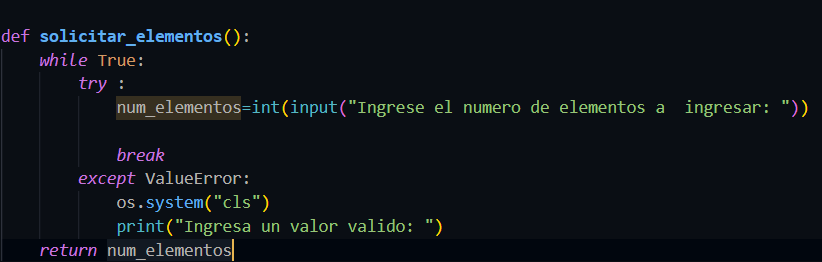
\includegraphics[width = .8\textwidth]{solicitar_elementos.png}
 		\captionof{figure}{\label{fig:IPN}Funcion para forzar al usuario a ingresar un numero entero} 
	\end{center} 
\end{figure}

Esta funcion es una que se va a compartir en varias funciones, ya que es fundamental que el usuario ingrese un valor de forma int, por lo cual, en el codigo esto es posible con un ciclo while, el cual se ejecuta mientras sea "True", es notable el uso de un "try" el cual tiene la funcion de "Intentar" obtener un valor entero, en caso de ingresar un valor de otro tipo, hace una limpieza del sistema con el comando "cls", y nuevamente se vuelve a pedir un valor valido, la forma de salir de este ciclo es ingresando un valor entero, para que se ejecute la sentencia "brea" y asi salir del ciclo while, para posteriormente devolver el numero de elementos
\\


\item Ingresar datos: Para llevar a cabo el proceso de solicitar datos, se implemento la Figura 2, la cual contiene la variable, "num\_elementos" donde usando la funcion del paso 1, esta almacena el numero de elementos a ingresar, posteriormente se declara la variable suma=0, e iniciamos un ciclo "for", el cual nos sirve para almacenar los n elementos que el usuario desea ingresar, notese el uso de un ciclo "while", muy similar al del paso 1, el cual se ejecutara mientras el usuario no ingrese un numero valido, este puede ser un valor de tipo entero o tipo flotante, en caso de ingresar un numero valido, el ciclo while se detendra para el valor de iteracion "i", ademas de que se asignara el espacio i-esimo de la matriz, tambien vamos a llevar a cabo la suma de cada valor ingresado con el comando suma=mat[i], el cual sumara cada elemento i-esimo que ingresemos.\\
Algo mas a destacar es la forma de creacion de un array, donde gracias a la libreria Numpy, la cual tenemos de forma abreviada "num", y usando uno de sus metodos ".empty" el cual nos crea una matris de n elementos iniciada en zeros

\begin{figure}[H]
	\begin{center}
	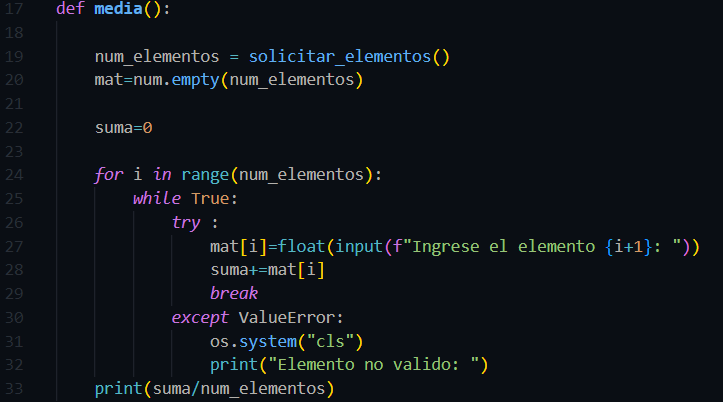
\includegraphics[width=.8\textwidth]{media.png}
	\captionof{figure}{\label{fig:Media}Funcion de la opcion media dentro del programa}
	\end{center}
\end{figure}


\item Calcular la media aritmetica: Para este ultimo paso es importante considererar la forma en la que implementamos el calculo, la cual a mi parecer es algo abstracta, debido que usamos la definicion de media aritmerica:  $ \bar{x} = \frac{1}{n} \sum_{i=1}^{n} x_i$\\
Es probable que Numpy tenga una funcion que haga esto de forma mas rapida. Una vez calculada la media aritmetica lo que resta es imprimir en pantalla el resultado.


\end{enumerate}

\item Desviacion Estandar\\
En esta funcion se busca preguntar al usuario una coleccion de datos y calcular su desviacion estandar usando la libreria Numpy
	\begin{enumerate}
		\item Ingreso numero de elementos: Este proceso se hace de la misma forma que en el caso anterior de la media aritmetica, recordando que partimos de la misma funcion, indicada en la Figura 1, de la misma forma necesitamos que ingrese un numero de tipo entero, por lo cual espero este paso no tiene ninguna complicacion
		\item Ingreso de datos: En la Figura 3, podemos observar la funcion desviacion\_estandar, la cual contiene similitud con el ejemplo anterior, creamos la matriz con ayuda de la libreria Numpy (num.empty()) la cual nos crea una matriz de n, elementos iniciados en ceros, posteriormente tenemos un ciclo for, donde se obliga al usuario a ingresar un elemento valido, ya sea de tipo entero (int) o de tipo flotante (float), esto gracias al ciclo while, el cual se terminara hasta ingresar un elemento valido
		\item Calculo desviacion estandar: Con ayuda de la libreria Numpy, podemos hacer uso de la funcion std(), la cual toma como argumento, un array y devuelve la desviacion estandar de esta coleccion de datos. Esto es de gran ayuda, debido a que la forma de calcular la desviacion estandar para n elementos  es de la forma $\sigma = \sqrt{\frac{1}{n} \sum_{i=1}^{n} (x_i - \bar{x})^2}
$. La cual resultaria muy tediosa de programar sin el uso de esta libreria. Para terminar mostramos en pantalla el resultado 
		\begin{figure}[H]
		\begin{center}
		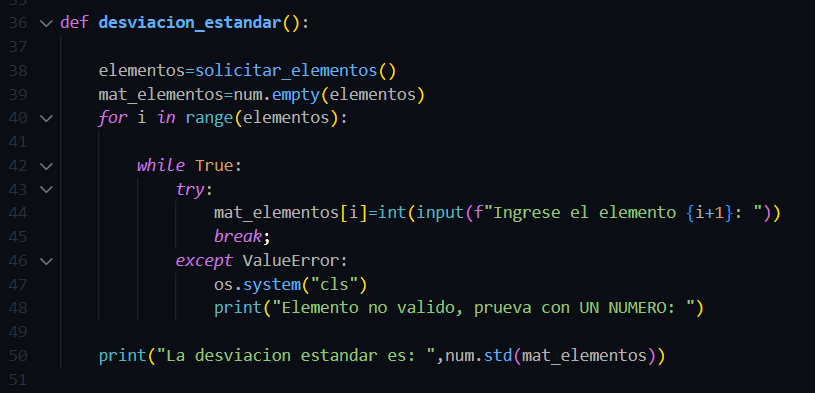
\includegraphics[width=.8\textwidth]{desviacion.png}
		\captionof{figure}{\label{fig:Media}Funcion de la opcion desviacion estandar}
		\end{center}
		\end{figure}

	\end{enumerate}

	
\item Burbuja:\\
En esta funcion se busca que el usuario ingrese el numero de elementos que desea obtener, usando la librerua Numpy, generar un arreglo semi aleatorio, del mismo tamaño de la entrada n, ademas de ordenar estos elementos usando el metodo burbuja
	\begin{enumerate}
	\item Solicitar el numero de elementos: En este paso seguimos usando la funcion indicada en la Figura 1, la cual nos proporcionara un numero entero de elementos
	\item Generar elementos: En esta parte del programa, nuevamente utilizaremos la libreria Numpy, usando el metodo rando.rand(num\_elementos), el cual devuelve un arrego con numeros aleatorios del tamaño indicado e imprime la matriz de elemetnos generados de forma aleatoria
	\item Ordenamiento: El ordenamiento burbuja como tal no lo encotre en la libreria, debido a que es uno de los menos efectivos y mas tardados, cuando hablamos de grandes cantidades de datos, para el programa se implento el ordenamiento burbuja, el cual consiste en iterar desde el primer elemento del array [i] iniciando los ciclos en i=0, y si este cumple que es mayor al elemento siguiente [i+1] se hace un intercambio de posiciones, es decir cambiamos el elemento mayor a la siguiente posicion, una vez que iteramos sobre todos los pares de elementos, el elemento mayor habra quedado en la parte final del array, de esta forma se puede iterar hasta ordenar todos los elementos, observe la Figura 5
		
	\begin{figure}[H]
		\begin{center}
		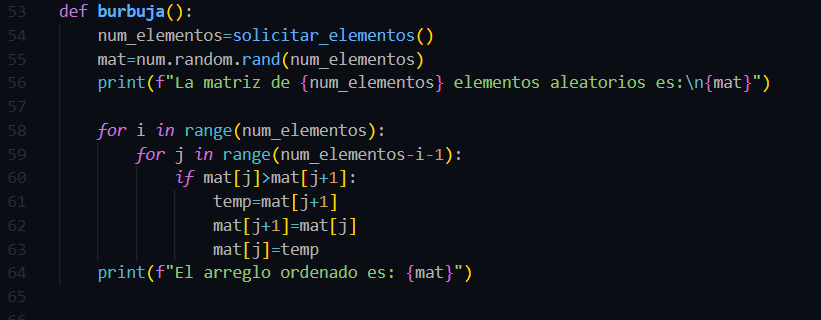
\includegraphics[width=.8\textwidth]{burbuja.png}
		\captionof{figure}{\label{fig:Media}Funcion de la opcion burbuja}
		\end{center}
		\end{figure}	
	\begin{figure}[H]
		\begin{center}
		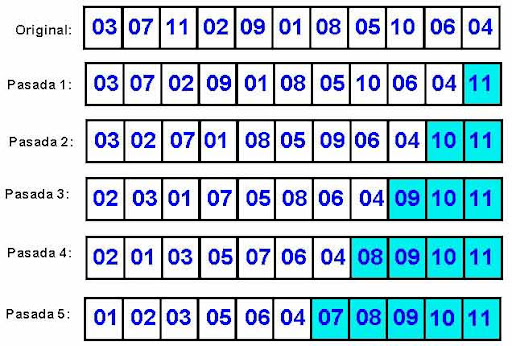
\includegraphics[width=.4\textwidth]{ejemplo_burbuja.jpg}
		\captionof{figure}{\label{fig:Media}Ejemplo de un ordenamiento burbuja}
		\end{center}
		\end{figure}	
	
	\end{enumerate}
	
	
	

\item Salir:\\
Para esta opcion dentro del menu, solo basta con imprimir un mensaje de despedida y finalizar el programa, se puede hacer de la siguiente manera: 

\begin{figure}[H]
		\begin{center}
		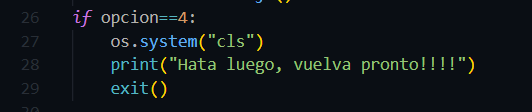
\includegraphics[width=.5\textwidth]{salir.png}
		\captionof{figure}{\label{fig:Media}Funcion de la opcion salir}
		\end{center}
		\end{figure}	

\end{itemize}

\begin{figure}[H]
	\begin{center}
 		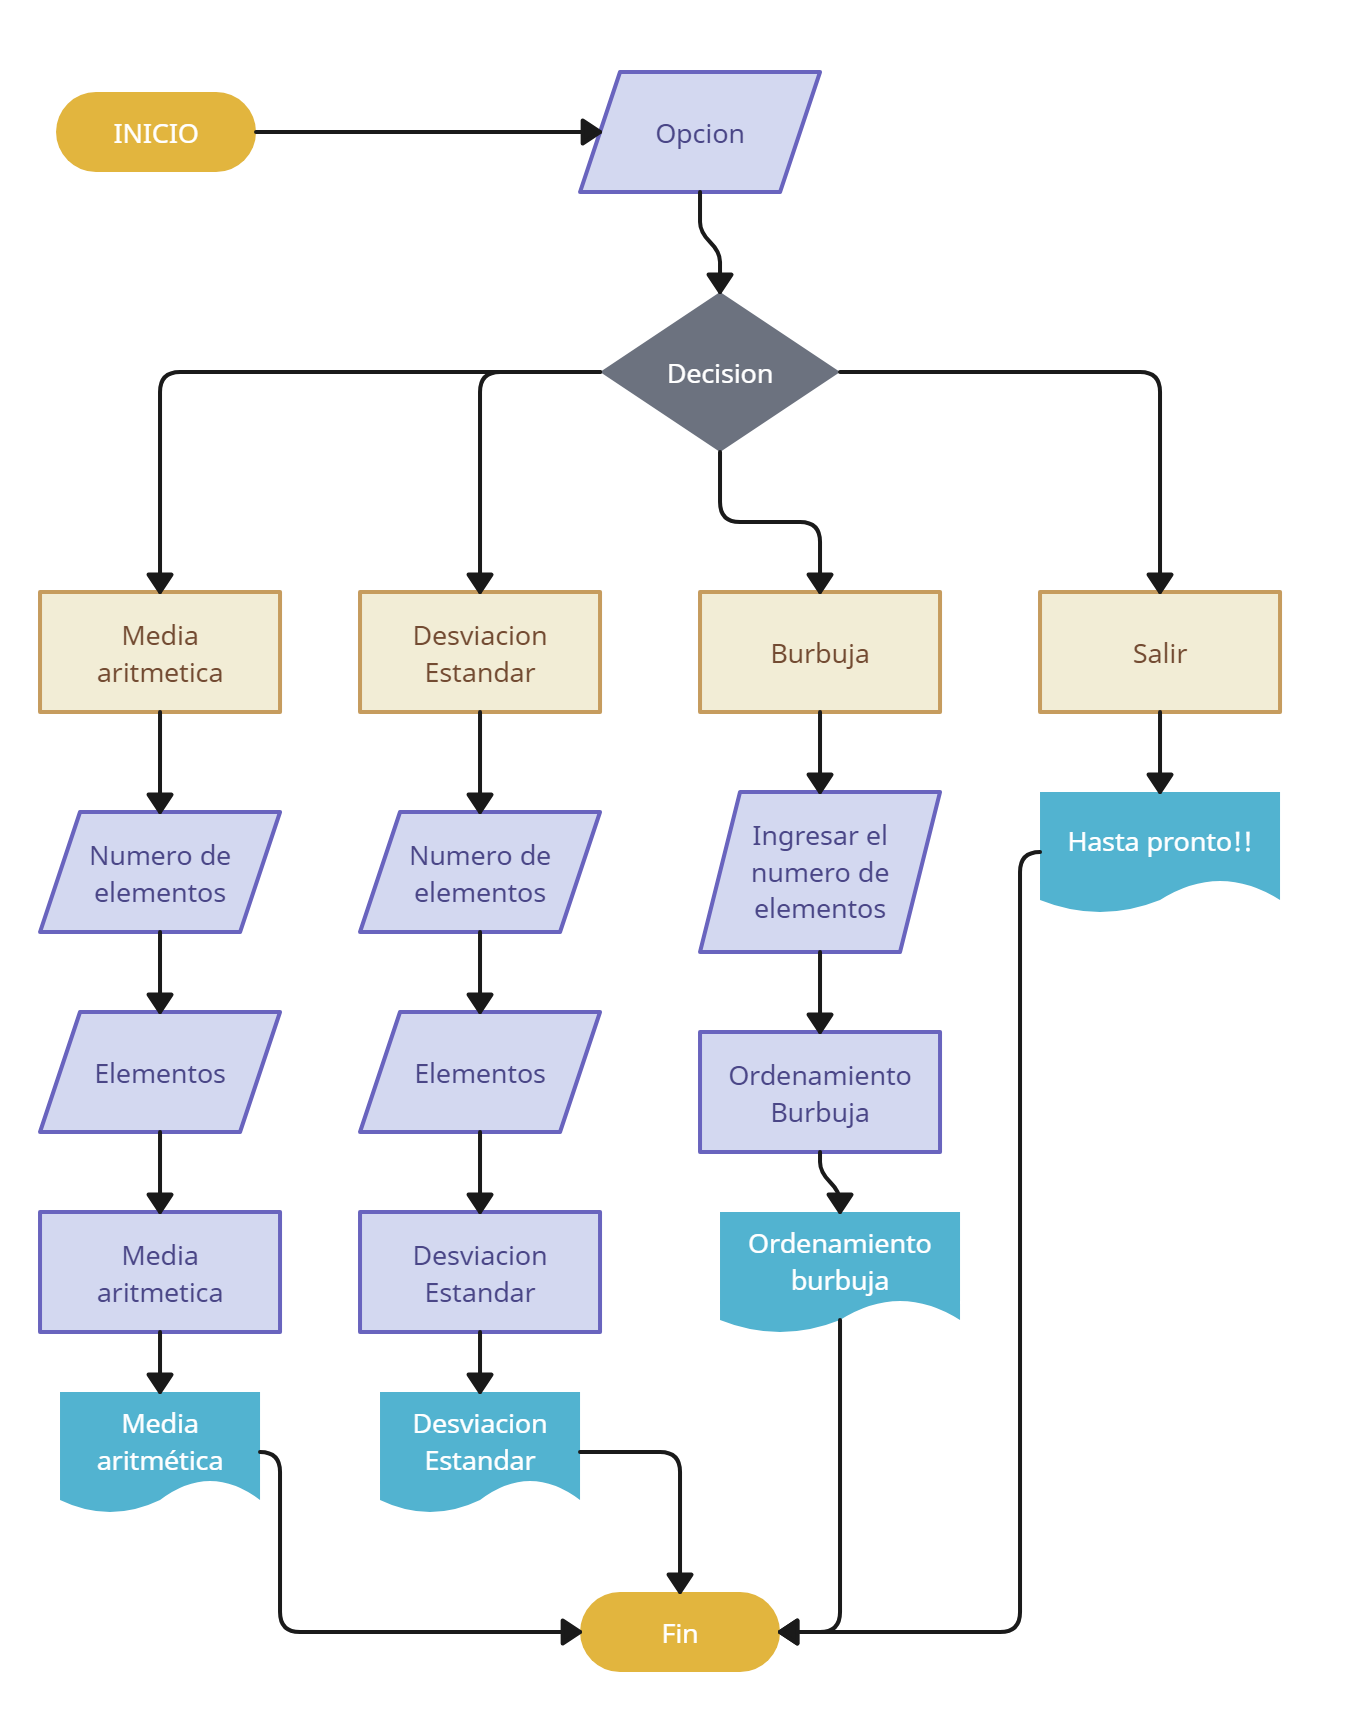
\includegraphics[width = .8\textwidth]{diagrama.png}
 		\captionof{figure}{\label{fig:IPN}Diagrama de flujo utilizado para el primer programa} 
	\end{center} 
\end{figure}
\newpage

\subsection{Sistemas de ecuaciones}

\begin{itemize}
\item Solucion al problema propuesto:\\
\begin{enumerate}
\item Analisis del problama:\\
a partir del sistema de ecuaciones proporcionada en el problema, el cual es el siguiente:\\

\[
\begin{aligned}
2x - 4y -3z &= 15 \\
x +5y -5z &= 5 \\
4x +2y +67z &= 20
\end{aligned}
\]
Donde podemos observar que
\[
A = \begin{bmatrix}
2 & -4 & -3 \\
1 & 5 & -5 \\
4 & 2 & 67 
\end{bmatrix}, \quad 
B = \begin{bmatrix}
15 \\
5 \\
20 
\end{bmatrix}
\]

\item Solucion:\\
Recordando que se esto se puede solucionar de la forma $X=A^{-1}*B$\\
En la Figura 8, podemos encontrar que utilizando la libreria Numpy, podemos declarar la matriz A, el vector B, con el metodo .array([]). Tambien notemos que para obtener la inversa de la matriz A, se usa otro metodo, el cual es .linalg.inv(A), el cual nos devuelve la matriz inversa\\
Finalmente para la solucion basta con usar la formula antes descrita, ya que contamos con todos los elementos necesarios para realizar el producto punto de $A^{-1}*B$, con el metodo .dot($A^{-1}$,B) es suficiente para que nos devuelva los resultados para cada variabke, los cuales se imprimen en pantalla
\begin{figure}[H]
		\begin{center}
 			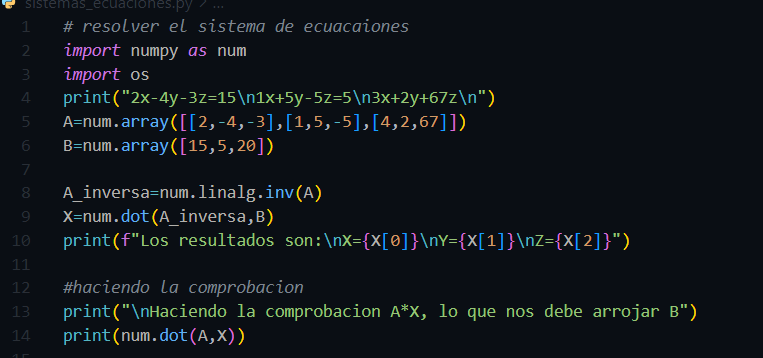
\includegraphics[width = .8\textwidth]{sistemae.png}
 			\captionof{figure}{\label{fig:IPN}Solucion al sistema de ecuaciones propuesto} 
		\end{center} 
	\end{figure}

\end{enumerate}
\item Modificacion para resolucion de sistemas 3x3:\\
	\begin{enumerate}
	\item Comenzamos preguntando al usuario si desea resolver un sistema de ecuaciones de 3x3, similar al ejemplo resuelto, obligando a responder con s/n gracias al ciclo while, de esta forma garantizamos que no "truene" el programa, en la figura 9, vemos que se usa la funcion de convertir a minusculas las opciones, con el fin de acepar tambien S/N
	
	\begin{figure}[H]
		\begin{center}
 			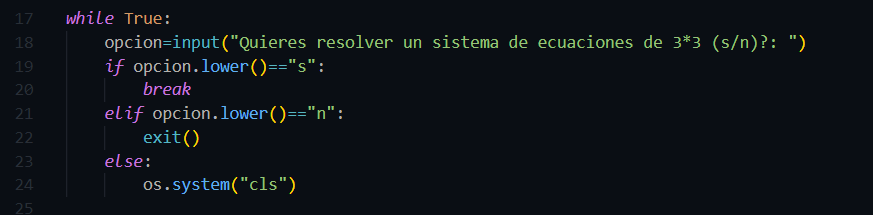
\includegraphics[width = .8\textwidth]{pregunta.png}
 			\captionof{figure}{\label{fig:IPN}funcion que solicita elementos en un arreglo 3x3} 
		\end{center} 
	\end{figure}
	
	\item Solicitar elementos del sistema: En este paso lo primero que hacemos es crear una matriz 3x3 de ceros, con ayuda de la libreria Numpy, usando el metodo .zeros((3,3)), la cual crea la matriz antes descrita. Iniciamos un ciclo for, el cual tiene la finalidad de solicitar los elementos, ademas de que estos elementos tienen que ser validos, esto es posible gracias al ciclo while y un try, el cual obliga al usuario a ingresar un elemento de tipo entero (int) o tipo float), en caso de ingresar otro tipo de dato el ciclo while se va a repetir hasta ingresar en elemento valido. 
	\begin{figure}[H]
		\begin{center}
 			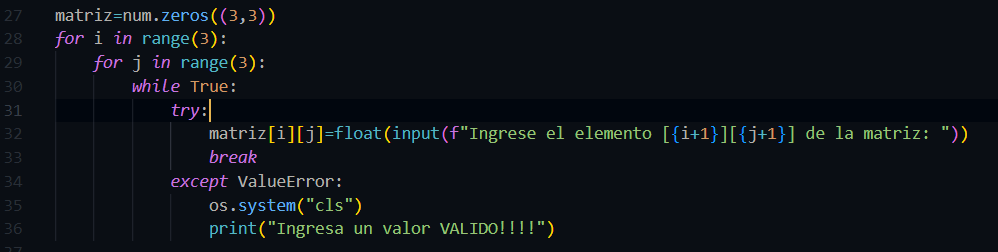
\includegraphics[width = .8\textwidth]{datos_mat.png}
 			\captionof{figure}{\label{fig:IPN}funcion para solicitar elementos de un vector con 3 elementos} 
		\end{center} 
	\end{figure}
	Esto fue para los valores de las variables (x,y,z).\\
	Para ingresar los valores del vector B, observemos la figura 11. Nuevamente usamos la el metodo .zeros(3) de la libreria numpy, ahora solo es un vector con 3 elemetnos, el cual guarda los resultados de cada ecuacion
	\begin{figure}[H]
		\begin{center}
 			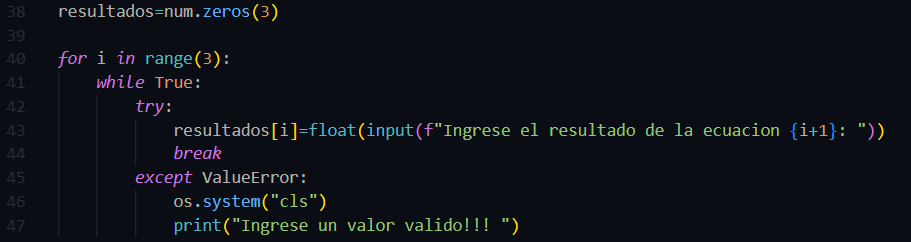
\includegraphics[width = .8\textwidth]{vec_b.png}
 			\captionof{figure}{\label{fig:IPN}funcion que pregunta al usuario si desea resolver un sistema} 
		\end{center} 
	\end{figure}
	\item Calculo resultados: \\
	En la figura 12, se observa que, el proceso es el mismo que en el ejemplo propuesto donde se busca la solucion por medio de la formula $ X=A^{-1}*B$, asi usando la libreria Numpy, para calcular la matriz inversa, y posteriormente imprimir el resultado en consola
	\begin{figure}[H]
		\begin{center}
 			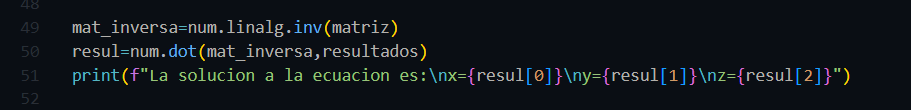
\includegraphics[width = .8\textwidth]{sol_mat.png}
 			\captionof{figure}{\label{fig:IPN}funcion para calcular el resultado de  la matriz ingresada} 
		\end{center} 
	\end{figure}
	
	
\end{enumerate}
\end{itemize}
	

\section{Ejecucion.}
\subsection{Entrada y Salida de Arreglos}
Ahora analizaremos el funcionamiento del programa\\
En la figura 13, se observa que nos muestra el menu, y nos pide que ingresemos 

\begin{figure}[H]
		\begin{center}
 			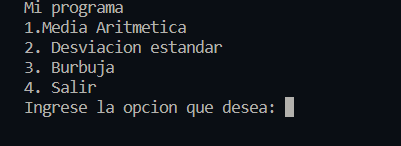
\includegraphics[width = .6\textwidth]{menu.png}
 			\captionof{figure}{\label{fig:IPN}Ejecucion del programa} 
		\end{center} 
	\end{figure}

Si intentamos ingresar algun elemento no valido, en consola, como se muestra en la figura 14. El programa volvera a mostrar el menu y  nuevamente pedira un elemento
	\begin{figure}[H]
		\begin{center}
 			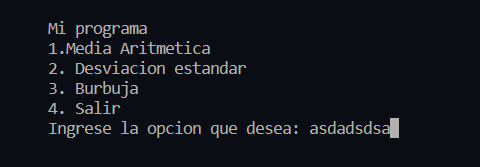
\includegraphics[width = .6\textwidth]{ingresa_val_erroneo.png}
 			\captionof{figure}{\label{fig:IPN}Ingreso de valores erroneos} 
		\end{center} 
	\end{figure}
	Esto ocaciona que el programa se vuelva a ejecutar hasta obtener una respuesta valida. 
	\begin{figure}[H]
		\begin{center}
 			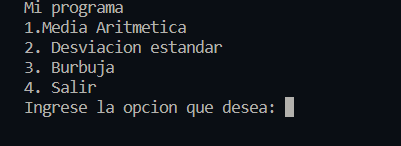
\includegraphics[width = .6\textwidth]{menu.png}
 			\captionof{figure}{\label{fig:IPN}Retorno del programa al ingresar un valor erroneo} 
		\end{center} 
	\end{figure}
Una vez que ingresemos un elemento valido,  por ejempllo, al ingresar el elemento 1, el cual nos deberia dirigir hacia la media aritmetica, veamos que sucede: Paa fines practicos vamos a ingresr 4 elementos, considerando que de la misma forma no nos dejara ingresar algun otro elemento que sea invalido. Vease la figura 16
 \\
 \\
 Ahora vamos a analizar la forma de ingresar los 4 elementos, tambien ingrese un valor no valido para ver la respuesta del programa, veamos en las siguientes imagenes el resultado
	\begin{figure}[H]
		\begin{center}
 			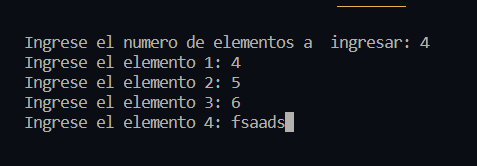
\includegraphics[width = .6\textwidth]{4_elementos.png}
 			\captionof{figure}{\label{fig:IPN}Ingreso de los 4 elementos} 
		\end{center} 
	\end{figure}

	\begin{figure}[H]
		\begin{center}
 			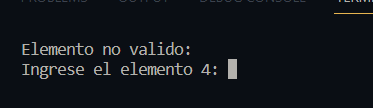
\includegraphics[width = .6\textwidth]{1_1.png}
 			\captionof{figure}{\label{fig:IPN}Respuesta al ingreso de un valor no valido} 
		\end{center} 
	\end{figure}
	Notamos que nos regresa un mensaje de elemento no valido. Ademas de nuevamente solicitar el elemento 4.\\
	Cuando ya ingresamos los datos correctos el programa nos arroja lo siguiente:
	\begin{figure}[H]
		\begin{center}
 			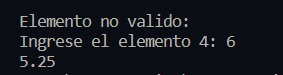
\includegraphics[width = .6\textwidth]{1_2.png}
 			\captionof{figure}{\label{fig:IPN}Resultado de la media aritmetica} 
		\end{center} 
	\end{figure}
	//Ahora solo mostraremos la ejecucion del programa, en cada una de las 3 opciones restantes, consideraremos las entradas de forma correcta, ya que en caso de ingresar un elemento no valido, simplemente nos volvera a pedir el elemento.
	\begin{itemize}
	\item Desviacion estandar
	\begin{figure}[H]
		\begin{center}
 			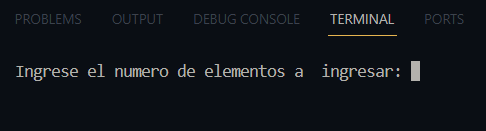
\includegraphics[width = .6\textwidth]{1_3.png}
 			\captionof{figure}{\label{fig:IPN}Nos pide el numero de elementos} 
		\end{center} 
	\end{figure}
	
	\begin{figure}[H]
		\begin{center}
 			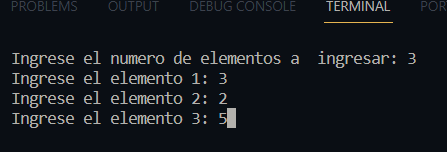
\includegraphics[width = .6\textwidth]{1_4.png}
 			\captionof{figure}{\label{fig:IPN}Ingreso de los elementos} 
		\end{center} 
	\end{figure}
	
	\begin{figure}[H]
		\begin{center}
 			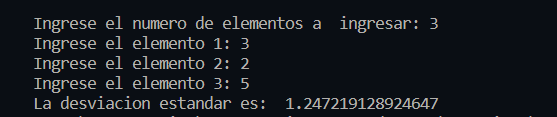
\includegraphics[width = .6\textwidth]{1_5.png}
 			\captionof{figure}{\label{fig:IPN}Resultado de la desviacion estandar} 
		\end{center} 
	\end{figure}
	
	\item Burbuja:\\
	Para esta funcion solo requiere el numero de elementos, ya que el resto lo realiza el programa (generar elementos y ordernarlos)
	\begin{figure}[H]
		\begin{center}
 			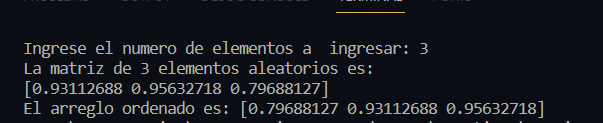
\includegraphics[width = .6\textwidth]{1_6.png}
 			\captionof{figure}{\label{fig:IPN}Metodo burbuja} 
		\end{center} 
	\end{figure}
	
	\item Salir:
	
	\begin{figure}[H]
		\begin{center}
 			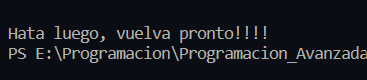
\includegraphics[width = .6\textwidth]{1_7.png}
 			\captionof{figure}{\label{fig:IPN}Opcion Salir} 
		\end{center} 
	\end{figure}
	
	\end{itemize}
	
\subsection{Sistema de ecuaciones}
Al ejecutar directamante el programa nos arroja lo siguiente en consola:\\
Veamos que tambien nos pregunta si queremos resolver un sistema independiente, vamos a poner que si  y seguir con el programa
	
	\begin{figure}[H]
		\begin{center}
 			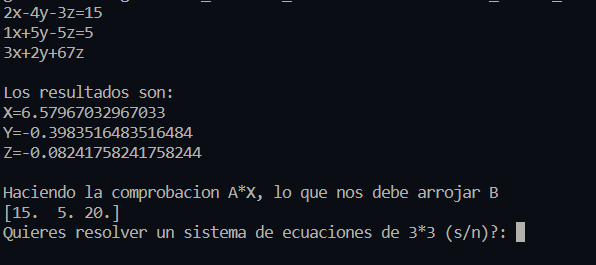
\includegraphics[width = .6\textwidth]{1_8.png}
 			\captionof{figure}{\label{fig:IPN}Resolucion del sistema de ecuaciones} 
		\end{center} 
	\end{figure}
	
	\begin{figure}[H]
		\begin{center}
 			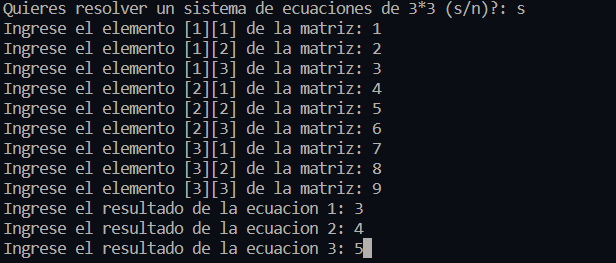
\includegraphics[width = .6\textwidth]{1_9.png}
 			\captionof{figure}{\label{fig:IPN}Ingresamos los valores del sistema de ecuaciones o la matriz, tambien ingresamos los resultados de cada ecuacion} 
		\end{center} 
	\end{figure}
	\begin{figure}[H]
		\begin{center}
 			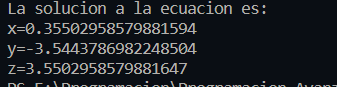
\includegraphics[width = .6\textwidth]{1_10.png}
 			\captionof{figure}{\label{fig:IPN}Resultado del sistema de ecuaciones} 
		\end{center} 
	\end{figure}
	
	


\section{Conclusiones.}
Al concluir esta practica e considerado que realizar este programa en python es bastante "sencillo" a comparacion de algun otro lenguaje como lo es C ó C++, que son los que ya que gracias a las librerias como Numpy se puede calcular la matriz inversa de forma inmediata.Asi que dando una opinion de forma generalizada python contiene herramientas que son muy poderosas, solo debemos encontrar la forma correcta de realizar una tarea. Esta practica sirve como introduccion  para lograr tener una mejor comprensio sobre este lenguaje de programacion, ya que una vez comprendido la logica de codificacion lo que resta es aprender la sintaxis, asi como nos sirve de introduccion para los siguientes temas, dandonos una muestra del poder de python junto con sus modulos.
\
%%%%%%% Bibliografía %%%%%%%%    

%\appendix  
%\clearpage % o \cleardoublepage
%\addappheadtotoc 
%\appendixpage

%\section{Anexos 1.}




%\section{Anexos 2.}


 

\end{document}
